\clearpage
\begin{examplebox}
\textbf{例1（给出两曲线，求焦角并验证不等式的等号）。}

椭圆 $E:x^2/16+y^2/12=1$，双曲线 $H:x^2-y^2/3=1$。
求它们的公共焦点、一个公共点 $P$，并求 $\theta=\angle F_1PF_2$。


\begin{center}
% Exact representative: F1=(-2,0), F2=(2,0), P=(2,3).
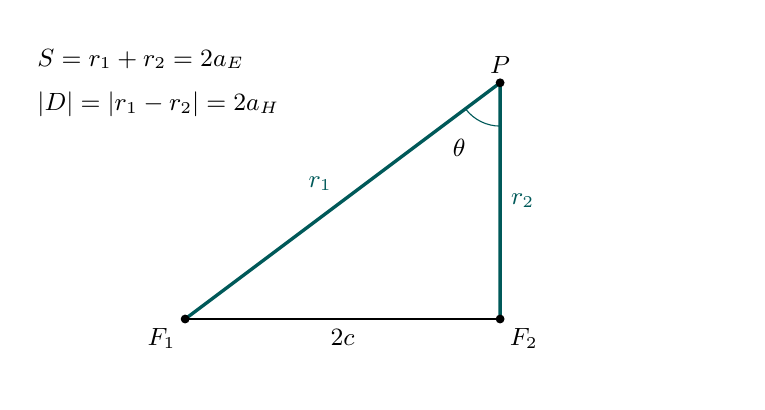
\begin{tikzpicture}[x=1cm,y=1cm,every node/.style={font=\small}]
\path[use as bounding box] (-4,-.8) rectangle (5,3.7);
\coordinate (L) at (-2,0); \coordinate (R) at (2,0); \coordinate (P) at (2,3);
\draw[very thick,teal!70!black] (L)--node[above left] {$r_1$} (P)--node[right] {$r_2$} (R);
\draw[thick] (L)--node[below] {$2c$} (R);
\draw[teal!70!black] (2,2.45) arc(-90:-143.130102:.55);
\node at (1.48,2.18) {$\theta$};
\foreach \v/\lab/\pos in {L/F_1/below left,R/F_2/below right,P/P/above}
  \fill (\v) circle(1.6pt) node[\pos] {$\lab$};
\node[align=left,anchor=west] at (-4,3) {$S=r_1+r_2=2a_E$\\[5pt] $|D|=|r_1-r_2|=2a_H$};
\end{tikzpicture}

\end{center}
图中三边正是本例的 $5,3,4$。
\textbf{识别信号：}给出两条标准方程，先查是否共焦，再把公共点
当作一个焦点三角形的第三顶点；已知三边就用余弦定理求角。

\textbf{解：}椭圆 $a_E=4$、$c=\sqrt{16-12}=2$；
双曲线 $a_H=1$、$c=\sqrt{1+3}=2$，故确实共焦，
$F_1=(-2,0),F_2=(2,0)$，且 $e_1=1/2,e_2=2$。
联立得 $x^2=4,y^2=9$（也可使用方法三的公共点坐标公式），
四个交点为 $(\pm2,\pm3)$；取 $P=(2,3)$，则
\[
 PF_1=5,\quad PF_2=3,\quad F_1F_2=4,
\quad\cos\theta=\frac{5^2+3^2-4^2}{2\cdot5\cdot3}=\frac35.
\]
\[
 \boxed{\theta=\arccos\frac35},\qquad\sin\theta=\frac45.
\]
验证：$1/e_1+1/e_2=2+1/2=5/2=2/(4/5)$，\textbf{恰好取等号}。
\textbf{图形解释：}$PF_2$ 是竖直线、$F_1F_2$ 是水平线，
所以直角在焦点 $F_2$，不是在 $P$；并且 $e_1e_2=1$。
\textbf{方法迁移：}焦点三角形的三边已知时，可以直接由余弦定理求焦角，
不必先求两条曲线的切线。
\end{examplebox}

\clearpage
\begin{examplebox}
\textbf{例2（已知离心率，快速反求焦角）。}

共焦椭圆、双曲线的离心率分别是
$e_1=1/2$、$e_2=3/2$，求公共点的焦点夹角 $\theta$。

\textbf{识别信号：}只给两条曲线的离心率，问题却要求 $\theta$；
优先使用已经消去焦半径的主公式，避免先联立求交点。
\textbf{最快解：}主公式
\[
 2=4(1-\cos\theta)+\frac49(1+\cos\theta).
\]
得 $18=40-32\cos\theta$，故
\[
 \boxed{\cos\theta=\frac{11}{16}},\qquad
 \boxed{\theta=\arccos\frac{11}{16}}.
\]
\textbf{为什么角度唯一？}余弦函数在 $(0,\pi)$ 上严格递减，
故 $\cos\theta=11/16$ 对应唯一的焦角。
\textbf{方法迁移：}四个公共点关于坐标轴成对称分布，
焦半径的\emph{和与差的绝对值}都相同，所以 $\theta$ 相同；
无需左右支分别推一遍。
\end{examplebox}

\clearpage
\begin{examplebox}
\textbf{例3（给定焦角，判断离心率是否可能）。}

已知 $\theta=60^\circ$，椭圆离心率 $e_1$ 可能为 $1/2$ 吗？
若 $e_1=1/\sqrt2$，求双曲线离心率 $e_2$。

\textbf{识别信号：}固定焦角，先检验离心率的\emph{存在性}，再求具体数值。
\textbf{解：}因为 $\sin30^\circ=1/2$、$\cos30^\circ=\sqrt3/2$，
主式为
\[
 \frac{1}{4e_1^2}+\frac{3}{4e_2^2}=1.
\]
当 $e_1=1/2$ 时第一项已等于 $1$，第二项严格大于 $0$，\textbf{不可能}。
当 $e_1=1/\sqrt2$ 时
\[
 \frac12+\frac{3}{4e_2^2}=1
\quad\Longrightarrow\quad \boxed{e_2=\sqrt{\frac32}>1}.
\]
\textbf{识别信号：}固定角度时必须 $e_1>\sin(\theta/2)$，
等号 $e_1=\sin(\theta/2)$ 无法对应有限的非退化双曲线。
\textbf{几何解释：}令 $T=c/e_2$。边界需要 $e_2\to\infty$，
即 $T\to0$；这是双曲线实半轴趋于零的退化极限，而不是一条正常双曲线。
\textbf{方法迁移：}“分母非零”只是第一层检查；
还必须检查所得 $e_1<1$、$e_2>1$，以及边界能否实际取到。
\end{examplebox}

\clearpage
\begin{examplebox}
\textbf{例4（高价值变式：固定焦角，何时达到推论的等号？）。}

已知共焦椭圆和双曲线的公共点满足 $\theta=60^\circ$。
求在所有符合条件的离心率对中 $1/e_1+1/e_2$ 的最大值。

\textbf{识别信号：}固定焦角，要求两个离心率倒数之\emph{和的最大值}，
应先用推论，再确认等号能否在 $0<e_1<1<e_2$ 内达到。
\textbf{解：}由推论有 $1/e_1+1/e_2\le2/\sin60^\circ=4/\sqrt3$。
等号条件给出
\[
 e_1=\tan30^\circ=\frac1{\sqrt3},\qquad
 e_2=\cot30^\circ=\sqrt3,
\]
两者符合 $0<e_1<1<e_2$，因此\textbf{等号可取}，
\[
 \boxed{\max\left(\frac1{e_1}+\frac1{e_2}\right)=\frac4{\sqrt3}}.
\]
\textbf{对照：}若 $\theta=120^\circ$，同一个柯西上界仍成立，
但要求 $e_1=\sqrt3>1$，与椭圆矛盾，\textbf{此时严格小于上界}。
\textbf{重要区别：}一个不等式给出的上界，不一定是实际可取到的最大值。
对 $\theta\ge90^\circ$，更精确的事实是
$1/e_1+1/e_2<2$，只能\emph{趋近} $2$，并不能达到。
推导见下一例；这是判断“最大值”和“上确界”时必须核查的边界。
\end{examplebox}

\clearpage
\begin{examplebox}
\textbf{例5（通用非直角焦点三角形：避免依赖 $3,4,5$ 特例）。}

设一组共焦椭圆、双曲线的半长轴、实半轴与半焦距分别是
$A=5,T=2,c=3$（确有 $T<c<A$），求公共点的焦角。

\textbf{识别信号：}给出共焦条件与轴长，不需要先联立求交点；
目标 $\theta$ 在同一个焦点三角形中。

\textbf{解：}定和 $r_1+r_2=10$、定差 $|r_1-r_2|=4$，
故两腰分别为 $7,3$，底边为 $2c=6$。
由余弦定理
\[
\cos\theta=\frac{7^2+3^2-6^2}{2\cdot7\cdot3}
=\frac{11}{21},\qquad
\boxed{\theta=\arccos\frac{11}{21}}.
\]
由于 $\cos\theta\ne0$，焦点三角形并非在 $P$ 处成直角。
又 $e_1=3/5,e_2=3/2$，有 $e_1e_2=9/10\ne1$，
所以焦角不等式在本例中为\emph{严格不等式}。

\textbf{方法迁移：}定和与定差确定两腰，焦距决定底边；
通常是一般斜三角形，不要把“等号直角图”当作定理的默认条件。
\end{examplebox}

\clearpage
\begin{examplebox}
\textbf{例6（锐角与钝角：柯西上界不等于最大值）。}

给定共焦椭圆、双曲线的焦角 $\theta$，问
$u+v=1/e_1+1/e_2$ 的\emph{最大值或上确界}。

\textbf{第一类：}$0<\theta<90^\circ$。柯西给出
$u+v\le2/\sin\theta$，并可取
$e_1=\tan(\theta/2)<1<\cot(\theta/2)=e_2$。
因此\emph{最大值}为 $2/\sin\theta$。

\textbf{第二类：}$90^\circ\le\theta<180^\circ$。
记 $s=\sin(\theta/2),t=\cos(\theta/2)$，则 $s^2\ge t^2$。
又 $u=1/e_1>1$、$0<v=1/e_2<1$，故 $u^2>v^2$。
于是
\[
\begin{aligned}
1=s^2u^2+t^2v^2
&\ge\frac{u^2+v^2}{2}\\
&>\frac{(u+v)^2}{4}.
\end{aligned}
\]
故\textbf{所有实际曲线}都满足 $u+v<2$。
固定该角度让 $e_1\to1^-$，由主公式可得 $e_2\to1^+$，
于是 $u+v\to2$，但两条曲线不能退化到 $e_1=e_2=1$。
所以此时\emph{没有最大值}，只有\emph{上确界} $2$。
\[
\boxed{\begin{array}{ll}
0<\theta<90^\circ:&\max(u+v)=2/\sin\theta;\\[2pt]
90^\circ\le\theta<180^\circ:&\sup(u+v)=2\ \text{（不可取到）}.
\end{array}}
\]
\textbf{方法迁移：}解最值题，要把“推导出上界”与“找出取等条件”
分成两步；端点不可取时，须区分最大值与上确界。
\end{examplebox}
